
% Default to the notebook output style

    


% Inherit from the specified cell style.




    
\documentclass{article}

    
    
    \usepackage{graphicx} % Used to insert images
    \usepackage{adjustbox} % Used to constrain images to a maximum size 
    \usepackage{color} % Allow colors to be defined
    \usepackage{enumerate} % Needed for markdown enumerations to work
    \usepackage{geometry} % Used to adjust the document margins
    \usepackage{amsmath} % Equations
    \usepackage{amssymb} % Equations
    \usepackage[mathletters]{ucs} % Extended unicode (utf-8) support
    \usepackage[utf8x]{inputenc} % Allow utf-8 characters in the tex document
    \usepackage{fancyvrb} % verbatim replacement that allows latex
    \usepackage{grffile} % extends the file name processing of package graphics 
                         % to support a larger range 
    % The hyperref package gives us a pdf with properly built
    % internal navigation ('pdf bookmarks' for the table of contents,
    % internal cross-reference links, web links for URLs, etc.)
    \usepackage{hyperref}
    \usepackage{longtable} % longtable support required by pandoc >1.10
    

    
    
    \definecolor{orange}{cmyk}{0,0.4,0.8,0.2}
    \definecolor{darkorange}{rgb}{.71,0.21,0.01}
    \definecolor{darkgreen}{rgb}{.12,.54,.11}
    \definecolor{myteal}{rgb}{.26, .44, .56}
    \definecolor{gray}{gray}{0.45}
    \definecolor{lightgray}{gray}{.95}
    \definecolor{mediumgray}{gray}{.8}
    \definecolor{inputbackground}{rgb}{.95, .95, .85}
    \definecolor{outputbackground}{rgb}{.95, .95, .95}
    \definecolor{traceback}{rgb}{1, .95, .95}
    % ansi colors
    \definecolor{red}{rgb}{.6,0,0}
    \definecolor{green}{rgb}{0,.65,0}
    \definecolor{brown}{rgb}{0.6,0.6,0}
    \definecolor{blue}{rgb}{0,.145,.698}
    \definecolor{purple}{rgb}{.698,.145,.698}
    \definecolor{cyan}{rgb}{0,.698,.698}
    \definecolor{lightgray}{gray}{0.5}
    
    % bright ansi colors
    \definecolor{darkgray}{gray}{0.25}
    \definecolor{lightred}{rgb}{1.0,0.39,0.28}
    \definecolor{lightgreen}{rgb}{0.48,0.99,0.0}
    \definecolor{lightblue}{rgb}{0.53,0.81,0.92}
    \definecolor{lightpurple}{rgb}{0.87,0.63,0.87}
    \definecolor{lightcyan}{rgb}{0.5,1.0,0.83}
    
    % commands and environments needed by pandoc snippets
    % extracted from the output of `pandoc -s`
    \DefineVerbatimEnvironment{Highlighting}{Verbatim}{commandchars=\\\{\}}
    % Add ',fontsize=\small' for more characters per line
    \newenvironment{Shaded}{}{}
    \newcommand{\KeywordTok}[1]{\textcolor[rgb]{0.00,0.44,0.13}{\textbf{{#1}}}}
    \newcommand{\DataTypeTok}[1]{\textcolor[rgb]{0.56,0.13,0.00}{{#1}}}
    \newcommand{\DecValTok}[1]{\textcolor[rgb]{0.25,0.63,0.44}{{#1}}}
    \newcommand{\BaseNTok}[1]{\textcolor[rgb]{0.25,0.63,0.44}{{#1}}}
    \newcommand{\FloatTok}[1]{\textcolor[rgb]{0.25,0.63,0.44}{{#1}}}
    \newcommand{\CharTok}[1]{\textcolor[rgb]{0.25,0.44,0.63}{{#1}}}
    \newcommand{\StringTok}[1]{\textcolor[rgb]{0.25,0.44,0.63}{{#1}}}
    \newcommand{\CommentTok}[1]{\textcolor[rgb]{0.38,0.63,0.69}{\textit{{#1}}}}
    \newcommand{\OtherTok}[1]{\textcolor[rgb]{0.00,0.44,0.13}{{#1}}}
    \newcommand{\AlertTok}[1]{\textcolor[rgb]{1.00,0.00,0.00}{\textbf{{#1}}}}
    \newcommand{\FunctionTok}[1]{\textcolor[rgb]{0.02,0.16,0.49}{{#1}}}
    \newcommand{\RegionMarkerTok}[1]{{#1}}
    \newcommand{\ErrorTok}[1]{\textcolor[rgb]{1.00,0.00,0.00}{\textbf{{#1}}}}
    \newcommand{\NormalTok}[1]{{#1}}
    
    % Define a nice break command that doesn't care if a line doesn't already
    % exist.
    \def\br{\hspace*{\fill} \\* }
    % Math Jax compatability definitions
    \def\gt{>}
    \def\lt{<}
    % Document parameters
    \title{Fasores}
    
    
    

    % Pygments definitions
    
\makeatletter
\def\PY@reset{\let\PY@it=\relax \let\PY@bf=\relax%
    \let\PY@ul=\relax \let\PY@tc=\relax%
    \let\PY@bc=\relax \let\PY@ff=\relax}
\def\PY@tok#1{\csname PY@tok@#1\endcsname}
\def\PY@toks#1+{\ifx\relax#1\empty\else%
    \PY@tok{#1}\expandafter\PY@toks\fi}
\def\PY@do#1{\PY@bc{\PY@tc{\PY@ul{%
    \PY@it{\PY@bf{\PY@ff{#1}}}}}}}
\def\PY#1#2{\PY@reset\PY@toks#1+\relax+\PY@do{#2}}

\expandafter\def\csname PY@tok@gp\endcsname{\let\PY@bf=\textbf\def\PY@tc##1{\textcolor[rgb]{0.00,0.00,0.50}{##1}}}
\expandafter\def\csname PY@tok@gi\endcsname{\def\PY@tc##1{\textcolor[rgb]{0.00,0.63,0.00}{##1}}}
\expandafter\def\csname PY@tok@gu\endcsname{\let\PY@bf=\textbf\def\PY@tc##1{\textcolor[rgb]{0.50,0.00,0.50}{##1}}}
\expandafter\def\csname PY@tok@ow\endcsname{\let\PY@bf=\textbf\def\PY@tc##1{\textcolor[rgb]{0.67,0.13,1.00}{##1}}}
\expandafter\def\csname PY@tok@ni\endcsname{\let\PY@bf=\textbf\def\PY@tc##1{\textcolor[rgb]{0.60,0.60,0.60}{##1}}}
\expandafter\def\csname PY@tok@gd\endcsname{\def\PY@tc##1{\textcolor[rgb]{0.63,0.00,0.00}{##1}}}
\expandafter\def\csname PY@tok@sc\endcsname{\def\PY@tc##1{\textcolor[rgb]{0.73,0.13,0.13}{##1}}}
\expandafter\def\csname PY@tok@cs\endcsname{\let\PY@it=\textit\def\PY@tc##1{\textcolor[rgb]{0.25,0.50,0.50}{##1}}}
\expandafter\def\csname PY@tok@vc\endcsname{\def\PY@tc##1{\textcolor[rgb]{0.10,0.09,0.49}{##1}}}
\expandafter\def\csname PY@tok@c\endcsname{\let\PY@it=\textit\def\PY@tc##1{\textcolor[rgb]{0.25,0.50,0.50}{##1}}}
\expandafter\def\csname PY@tok@m\endcsname{\def\PY@tc##1{\textcolor[rgb]{0.40,0.40,0.40}{##1}}}
\expandafter\def\csname PY@tok@cm\endcsname{\let\PY@it=\textit\def\PY@tc##1{\textcolor[rgb]{0.25,0.50,0.50}{##1}}}
\expandafter\def\csname PY@tok@go\endcsname{\def\PY@tc##1{\textcolor[rgb]{0.53,0.53,0.53}{##1}}}
\expandafter\def\csname PY@tok@nv\endcsname{\def\PY@tc##1{\textcolor[rgb]{0.10,0.09,0.49}{##1}}}
\expandafter\def\csname PY@tok@o\endcsname{\def\PY@tc##1{\textcolor[rgb]{0.40,0.40,0.40}{##1}}}
\expandafter\def\csname PY@tok@sb\endcsname{\def\PY@tc##1{\textcolor[rgb]{0.73,0.13,0.13}{##1}}}
\expandafter\def\csname PY@tok@si\endcsname{\let\PY@bf=\textbf\def\PY@tc##1{\textcolor[rgb]{0.73,0.40,0.53}{##1}}}
\expandafter\def\csname PY@tok@sd\endcsname{\let\PY@it=\textit\def\PY@tc##1{\textcolor[rgb]{0.73,0.13,0.13}{##1}}}
\expandafter\def\csname PY@tok@ss\endcsname{\def\PY@tc##1{\textcolor[rgb]{0.10,0.09,0.49}{##1}}}
\expandafter\def\csname PY@tok@il\endcsname{\def\PY@tc##1{\textcolor[rgb]{0.40,0.40,0.40}{##1}}}
\expandafter\def\csname PY@tok@c1\endcsname{\let\PY@it=\textit\def\PY@tc##1{\textcolor[rgb]{0.25,0.50,0.50}{##1}}}
\expandafter\def\csname PY@tok@no\endcsname{\def\PY@tc##1{\textcolor[rgb]{0.53,0.00,0.00}{##1}}}
\expandafter\def\csname PY@tok@nd\endcsname{\def\PY@tc##1{\textcolor[rgb]{0.67,0.13,1.00}{##1}}}
\expandafter\def\csname PY@tok@bp\endcsname{\def\PY@tc##1{\textcolor[rgb]{0.00,0.50,0.00}{##1}}}
\expandafter\def\csname PY@tok@sx\endcsname{\def\PY@tc##1{\textcolor[rgb]{0.00,0.50,0.00}{##1}}}
\expandafter\def\csname PY@tok@gr\endcsname{\def\PY@tc##1{\textcolor[rgb]{1.00,0.00,0.00}{##1}}}
\expandafter\def\csname PY@tok@kr\endcsname{\let\PY@bf=\textbf\def\PY@tc##1{\textcolor[rgb]{0.00,0.50,0.00}{##1}}}
\expandafter\def\csname PY@tok@k\endcsname{\let\PY@bf=\textbf\def\PY@tc##1{\textcolor[rgb]{0.00,0.50,0.00}{##1}}}
\expandafter\def\csname PY@tok@kp\endcsname{\def\PY@tc##1{\textcolor[rgb]{0.00,0.50,0.00}{##1}}}
\expandafter\def\csname PY@tok@mo\endcsname{\def\PY@tc##1{\textcolor[rgb]{0.40,0.40,0.40}{##1}}}
\expandafter\def\csname PY@tok@gs\endcsname{\let\PY@bf=\textbf}
\expandafter\def\csname PY@tok@sh\endcsname{\def\PY@tc##1{\textcolor[rgb]{0.73,0.13,0.13}{##1}}}
\expandafter\def\csname PY@tok@kn\endcsname{\let\PY@bf=\textbf\def\PY@tc##1{\textcolor[rgb]{0.00,0.50,0.00}{##1}}}
\expandafter\def\csname PY@tok@kt\endcsname{\def\PY@tc##1{\textcolor[rgb]{0.69,0.00,0.25}{##1}}}
\expandafter\def\csname PY@tok@vg\endcsname{\def\PY@tc##1{\textcolor[rgb]{0.10,0.09,0.49}{##1}}}
\expandafter\def\csname PY@tok@nt\endcsname{\let\PY@bf=\textbf\def\PY@tc##1{\textcolor[rgb]{0.00,0.50,0.00}{##1}}}
\expandafter\def\csname PY@tok@mi\endcsname{\def\PY@tc##1{\textcolor[rgb]{0.40,0.40,0.40}{##1}}}
\expandafter\def\csname PY@tok@kc\endcsname{\let\PY@bf=\textbf\def\PY@tc##1{\textcolor[rgb]{0.00,0.50,0.00}{##1}}}
\expandafter\def\csname PY@tok@mh\endcsname{\def\PY@tc##1{\textcolor[rgb]{0.40,0.40,0.40}{##1}}}
\expandafter\def\csname PY@tok@na\endcsname{\def\PY@tc##1{\textcolor[rgb]{0.49,0.56,0.16}{##1}}}
\expandafter\def\csname PY@tok@mf\endcsname{\def\PY@tc##1{\textcolor[rgb]{0.40,0.40,0.40}{##1}}}
\expandafter\def\csname PY@tok@w\endcsname{\def\PY@tc##1{\textcolor[rgb]{0.73,0.73,0.73}{##1}}}
\expandafter\def\csname PY@tok@ne\endcsname{\let\PY@bf=\textbf\def\PY@tc##1{\textcolor[rgb]{0.82,0.25,0.23}{##1}}}
\expandafter\def\csname PY@tok@nc\endcsname{\let\PY@bf=\textbf\def\PY@tc##1{\textcolor[rgb]{0.00,0.00,1.00}{##1}}}
\expandafter\def\csname PY@tok@nf\endcsname{\def\PY@tc##1{\textcolor[rgb]{0.00,0.00,1.00}{##1}}}
\expandafter\def\csname PY@tok@nl\endcsname{\def\PY@tc##1{\textcolor[rgb]{0.63,0.63,0.00}{##1}}}
\expandafter\def\csname PY@tok@gt\endcsname{\def\PY@tc##1{\textcolor[rgb]{0.00,0.27,0.87}{##1}}}
\expandafter\def\csname PY@tok@sr\endcsname{\def\PY@tc##1{\textcolor[rgb]{0.73,0.40,0.53}{##1}}}
\expandafter\def\csname PY@tok@gh\endcsname{\let\PY@bf=\textbf\def\PY@tc##1{\textcolor[rgb]{0.00,0.00,0.50}{##1}}}
\expandafter\def\csname PY@tok@vi\endcsname{\def\PY@tc##1{\textcolor[rgb]{0.10,0.09,0.49}{##1}}}
\expandafter\def\csname PY@tok@s1\endcsname{\def\PY@tc##1{\textcolor[rgb]{0.73,0.13,0.13}{##1}}}
\expandafter\def\csname PY@tok@nb\endcsname{\def\PY@tc##1{\textcolor[rgb]{0.00,0.50,0.00}{##1}}}
\expandafter\def\csname PY@tok@s2\endcsname{\def\PY@tc##1{\textcolor[rgb]{0.73,0.13,0.13}{##1}}}
\expandafter\def\csname PY@tok@nn\endcsname{\let\PY@bf=\textbf\def\PY@tc##1{\textcolor[rgb]{0.00,0.00,1.00}{##1}}}
\expandafter\def\csname PY@tok@cp\endcsname{\def\PY@tc##1{\textcolor[rgb]{0.74,0.48,0.00}{##1}}}
\expandafter\def\csname PY@tok@s\endcsname{\def\PY@tc##1{\textcolor[rgb]{0.73,0.13,0.13}{##1}}}
\expandafter\def\csname PY@tok@se\endcsname{\let\PY@bf=\textbf\def\PY@tc##1{\textcolor[rgb]{0.73,0.40,0.13}{##1}}}
\expandafter\def\csname PY@tok@ge\endcsname{\let\PY@it=\textit}
\expandafter\def\csname PY@tok@kd\endcsname{\let\PY@bf=\textbf\def\PY@tc##1{\textcolor[rgb]{0.00,0.50,0.00}{##1}}}
\expandafter\def\csname PY@tok@err\endcsname{\def\PY@bc##1{\setlength{\fboxsep}{0pt}\fcolorbox[rgb]{1.00,0.00,0.00}{1,1,1}{\strut ##1}}}

\def\PYZbs{\char`\\}
\def\PYZus{\char`\_}
\def\PYZob{\char`\{}
\def\PYZcb{\char`\}}
\def\PYZca{\char`\^}
\def\PYZam{\char`\&}
\def\PYZlt{\char`\<}
\def\PYZgt{\char`\>}
\def\PYZsh{\char`\#}
\def\PYZpc{\char`\%}
\def\PYZdl{\char`\$}
\def\PYZhy{\char`\-}
\def\PYZsq{\char`\'}
\def\PYZdq{\char`\"}
\def\PYZti{\char`\~}
% for compatibility with earlier versions
\def\PYZat{@}
\def\PYZlb{[}
\def\PYZrb{]}
\makeatother


    % Exact colors from NB
    \definecolor{incolor}{rgb}{0.0, 0.0, 0.5}
    \definecolor{outcolor}{rgb}{0.545, 0.0, 0.0}



    
    % Prevent overflowing lines due to hard-to-break entities
    \sloppy 
    % Setup hyperref package
    \hypersetup{
      breaklinks=true,  % so long urls are correctly broken across lines
      colorlinks=true,
      urlcolor=blue,
      linkcolor=darkorange,
      citecolor=darkgreen,
      }
    % Slightly bigger margins than the latex defaults
    
    \geometry{verbose,tmargin=1in,bmargin=1in,lmargin=1in,rmargin=1in}
    
    

    \begin{document}
    
    
    \maketitle
    
    

    

    \section{Fasores}


    Contenido


    \subsection{Introducción}


    Un fasor es una representación de una oscilación a través de un número
complejo. En física e ingeniería,un vector de fase o fasor, es una
representación de una función sinusoidal con una amplitud (A),
frecuencia ($\omega$), fase ($\theta$) y es invariente en el tiempo.

Segun la identidad de Euler se tiene

\begin{equation}
A\cdot \cos(\omega t + \theta) = A \cdot \frac{e^{i(\omega t + \theta)} + e^{-i(\omega t + \theta)}},
\end{equation}

seleccionando únicamente la parte real

\begin{align}
A\cdot \cos(\omega t + \theta) &= \operatorname{Re} \left\{ A\cdot e^{i(\omega t + \theta)}\right\} \\
&= \operatorname{Re} \left\{ A e^{i\theta} \cdot e^{i\omega t}\right\}.
\end{align}

El termino fasor se puede referir a $Ae^{i\theta}e^{i \omega t} $ o
simplemente a la constante compleja, $A e^{i\theta}\, $. Es importante
notar que

\[
\cos(\omega t)= \sin (\omega t + 90º)=\operatorname{Re} \left\{ A e^{i\theta+\frac{\pi}{2}} \cdot e^{i\omega t}\right\},
\] por lo que se puede afirmar que $A\cos(\omega t+ \theta)$ puede
representar a cualquier señal oscilatoria periodica simple.


    \subsection{Derivación e Integración del fasor}


    La derivada en tiempo de un fasor es

\begin{align*}
\operatorname{Re}\left\{\frac{d}{d t}(A e^{i\theta} \cdot e^{i\omega t})\right\}
&= \operatorname{Re}\{A e^{i\theta} \cdot i\omega e^{i\omega t}\} \\
&= \operatorname{Re}\{A e^{i\theta} \cdot e^{i\pi/2} \omega e^{i\omega t}\} \\
&= \operatorname{Re}\{\omega A e^{i(\theta + \pi/2)} \cdot e^{i\omega t}\} \\
&= \omega A\cdot \cos(\omega t + \theta + \pi/2)
\end{align*}

Por lo tanto, en la representación fasorial la derivación en tiempo de
una señal senoidal es soloamente multiplar el fasor por la constante,

\begin{equation}
i \omega = (e^{i\pi/2} \cdot \omega)\,.
\end{equation}

De forma similar, \textbf{integrar en tiempo} un fasor corresponde a la
multiplicación por la constante

\begin{equation}
\frac{1}{i\omega} = \frac{e^{-i\pi/2}}{\omega}.
\end{equation}

El factor dependiendte del tiempo, $e^{i\omega t}\,,$ no es afectado.


    \subsection{Serie de Fourier}


    Una serie de Fourier es una \emph{serie infinita} que converge
puntualmente a una función periódica y continua a trozos (o por partes)
Si $f(t)$ es una función (o señal) periódica y su período es $T$, la
serie de Fourier asociada a $f(t)$ es:

\begin{equation}
f(t) \sim \frac{a_0}{2} + \sum_{n=1}^\infty\left[a_n\cos\frac{2n\pi}{T}t + b_n\sin\frac{2n\pi}{T}t\right]
\end{equation}

Donde $a_0$, $a_n$ y $b_n$ son los coeficientes de Fourier que toman los
valores:

\[
a_0 = \frac{2}{T} \int \limits_{-T/2}^{T/2} f(t) dt, \qquad a_n = \frac{2}{T} \int_{-T/2}^{T/2} f(t) \cos \left( \frac{2n \pi}{T} t \right) dt, \qquad b_n=\frac{2}{T} \int_{-T/2}^{T/2} f(t) \sin \left(\frac{2n\pi}{T}t\right) dt.
\]

En ocasiones es más útil conocer la amplitud y la fase en términos
cosinusoidales en lugar de amplitudes cosinusoidales y sinusoidal. Otra
forma de expresar la compleja forma de la serie de Fourier es:

\begin{equation}
f(t)=A_0+\sum_{n=1}^{\infty} A_{n}\,\cos({{\omega_n}t}-\theta_n)
\end{equation}

donde

\begin{align*}
A_0=&\frac{a_0}{2} \\
A_n=&\sqrt{a^2_n+b^2_n} \\
\theta_n=&\tan^{-1}\frac{b_n}{a_n}
\end{align*}

Por la identidad de Euler, las fórmulas de arriba pueden expresarse
también en su forma compleja:

\begin{equation}
f(t) \sim \sum_{n=-\infty}^{\infty} c_{n}\,e^{2\pi i\frac{n}{T}t}.
\end{equation}

Los coeficientes ahora serían: \[
c_n=\frac{1}{T}\int_{-T/2}^{T/2} f(t)e^{-2\pi i\frac {n}{T}t}\,dt.
\]


    \subsubsection{Ejemplo}


    Considere

\[
f(t)=\cos(2\pi20t)+2\sin(2\pi10t)+1.5\cos(2\pi40t)
\]

\[
C_{n}=\frac{1}{N}\sum_{i=0}^{i=N-1}y(i)e^{-2\pi i\frac {nt}{T}}.
\]


    \begin{center}
    \adjustimage{max size={0.9\linewidth}{0.9\paperheight}}{Fasores_files/Fasores_10_0.png}
    \end{center}
    { \hspace*{\fill} \\}
    

    \section{Analisis de circuitos con fasores}


    Consider el circuito que se muestra en la siguiente figura

\begin{figure}[htbp]
\centering
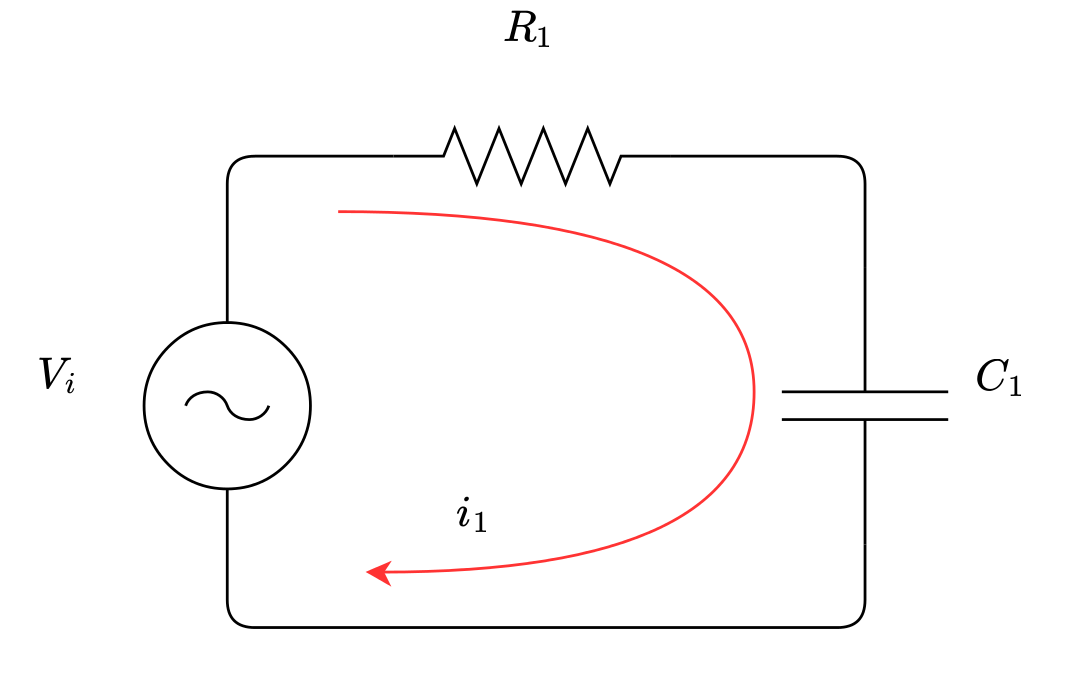
\includegraphics{images/rcserie.png}
\caption{Circuito RC serie}
\end{figure}

utilizando las leyes de krichof se tiene que \[
i_{R}=i_{C}
\] utilizando las ley de ohm y las propiedades del capcitor de tiene \[
\frac{V_{i}(t)-V_{C}(t)}{R}=C\frac{dV_{C}(t)}{dt}
\] despejando se tiene

\begin{equation}\label{eq:cirrc}
C\frac{dV_{C}(t)}{dt}+\frac{V_{C}(t)}{R}=\frac{V_{i}(t)}{R}
\end{equation}

Considerando $V_{i}(t)$ como

\[
V_i(t) = V_P\cdot \cos(\omega t + \theta),
\]

si se considera su representación en fasores

\begin{align*} 
V_i(t) =& \operatorname{Re} \{V_i \cdot e^{i\omega t}\} \\  
V_C(t) =& \operatorname{Re} \{V_c \cdot e^{i\omega t}\}
\end{align*}

donde el fasor $V_i = V_P e^{i\theta},$ y el fasor $V_c$ es desconocido
y es la variable a encontrar. En notación fasorial la expresión
\eqref{eq:cirrc} es

\[
i \omega V_c + \frac{1}{RC} V_c = \frac{1}{RC}V_i
\] Resolviendo para el fasor de $V_{C}$ se tiene

\[
V_c = \frac{1}{1 + i \omega RC} \cdot (V_i) = \frac{1-i\omega R C}{1+(\omega R C)^2} \cdot (V_P e^{i\theta})
\]

El factor que multiplica al fasor $V_i$ representa la diferencia en
amplitud y fase de $V_C(t)$ respecto a $V_{i}(t)$. Sin embargo, la
representación de dicho factor en la expresión anterior resulta
complicada de resolver como fasor, por lo que si se considera su
representación polar se tiene

\[
\frac{1}{\sqrt{1 + (\omega RC)^2}}\cdot e^{-i \phi(\omega)}
\] donde \[
\phi(\omega) = \arctan(\omega RC).
\] Considerando las expresiones anteriores se tiene

\begin{equation}
V_C(t) = \frac{1}{\sqrt{1 + (\omega RC)^2}}\cdot V_P \cos(\omega t + \theta- \phi(\omega)) 
\end{equation}

Considerando la ganancia del sitema definida como la razón entre la
señal de salida y la señal de entrada, en el circuito RC se tiene que la
ganacia es

\begin{equation}
\frac{V_{C}}{V_{i}}=\frac{1}{\sqrt{1 + (\omega RC)^2}}\cdot e^{-i \phi(\omega)}
\end{equation}

de la expresión anterior se tiene que la ganacia nos indica que
$V_C=V_i$ cuando $\omega=0$, y teoricamente $V_C=0$ cuando
$\omega=\infty$


    \begin{center}
    \adjustimage{max size={0.9\linewidth}{0.9\paperheight}}{Fasores_files/Fasores_13_0.png}
    \end{center}
    { \hspace*{\fill} \\}
    

    \subsection{Decibel}


    El decibelio (dB) es una unidad logarítmica utilizada para expresar la
relación entre dos valores de una cantidad física, a menudo potencia o
intensidad. Una de estas cantidades es a menudo el valor de referencia,
y en este caso el decibelio se puede utilizar para expresar el nivel
absoluto de la cantidad física. El decibel también se utiliza comúnmente
como una medida de la ganancia o de atenuación, la relación de entrada y
salida de potencias de un sistema, o de factores individuales que
contribuyen a este tipo de coeficientes.

\[
L_\mathrm{dB} = 10 \log_{10} \bigg(\frac{P_1}{P_0}\bigg) \,
\]

En circuitos eléctricos, la potencia disipada es normalmente
proporcional al cuadrado del voltaje o corriente cuando la impedancia se
mantiene constante. Tomando el voltaje como un ejemplo, esto conduce a
la ecuación:

\[
G_\mathrm{dB} =20 \log_{10} \left (\frac{V_o}{V_i} \right ) \quad \mathrm \quad
\]


    \begin{center}
    \adjustimage{max size={0.9\linewidth}{0.9\paperheight}}{Fasores_files/Fasores_16_0.png}
    \end{center}
    { \hspace*{\fill} \\}
    

    \begin{center}
    \adjustimage{max size={0.9\linewidth}{0.9\paperheight}}{Fasores_files/Fasores_17_0.png}
    \end{center}
    { \hspace*{\fill} \\}
    
    Pagina escrita en Ipython por \emph{Manuel Moisés Miranda Velasco}


    % Add a bibliography block to the postdoc
    
    
    
    \end{document}
